\documentclass[twoside]{article}
\usepackage{exam}
\usepackage{enumitem}
\usepackage{verbatim}



\graphicspath{
    {figures/}
}

\pagestyle{myheadings}
\markboth{}{{\large Name: }\sp{4in}}
\nonstopmode

% For Python code
\lstset{%
  language=Python,
  basicstyle=\ttfamily,
  showstringspaces=false
  keywordstyle=\color{black},
  commentstyle=\color{black},
  stringstyle=\color{black},
}

\def\semester{Summer 2019}

\newcommand{\bubble}{\raisebox{-0.3ex}{
\includegraphics[height=2ex]{oval.png}}}
\newcommand{\checkbox}{\raisebox{-0.3ex}{
\includegraphics[height=2ex]{square.png}}{\hskip 0.05in}}
\newcommand{\filledbubble}{\raisebox{-0.3ex}{
\includegraphics[height=2ex]{oval-filled.png}}}
\newcommand{\filledsquare}{\raisebox{-0.3ex}{
\includegraphics[height=2ex]{square-filled.png}}}
\newcommand{\lsi}{\lstinline}
\newcommand{\bkshort}{\underline{\qquad\qquad\qquad}\lsi}
\newcommand{\bk}{\underline{\qquad\qquad\qquad\qquad\qquad}\lsi}
\newcommand{\bkmed}{\underline{\qquad\qquad\qquad\qquad\qquad\qquad\qquad\qquad}\lsi}
\newcommand{\bklong}{\hrulefill}
\newcommand{\nlvs}{\newline\vskip 0.1in}

% Uncomment next line to generate pdf with solutions
% \newcommand{\issolution}{}

%%% Showing solutions %%%%%%%%%%%%%%%%%%%%%%%%%%%%%%%%%%%%%%%%%%%%%%%%%%%%%%%%%
\ifdef{\issolution}{%
    \newcommand{\solution}[1]{{\color{red}#1}}
    \newcommand{\solutioncircle}[1]{{\color{red}#1}}
    \newcommand{\solutionbubble}[0]{\filledbubble}
    \newcommand{\solutionbox}[0]{\filledsquare}
    \newcommand{\solutionimage}[2]{{\color{red}#2}}  % First arg is question, second is solution
    \newcommand{\versioned}[2]{{\color{red}#2}} % First arg is question, second is solution
}{%
    \newcommand\solution[1]{} % excludes
    \newcommand{\solutioncircle}[1]{#1} % don't color text but still display it
    \newcommand{\solutionbubble}[0]{\bubble}
    \newcommand{\solutionbox}[0]{\checkbox}
    \newcommand{\solutionimage}[2]{#1} % First arg is question, second is solution
    \newcommand{\versioned}[2]{#1} % First arg is question, second is solution
}

\newcommand{\TBD}{{\color{red}{ TBD }}}

%%% Document %%%%%%%%%%%%%%%%%%%%%%%%%%%%%%%%%%%%%%%%%%%%%%%%%%%%%%%%%%%%%%%%%%

\title{\sc Final Exam \solution{Solutions}}

\begin{document}
\thispagestyle{empty}
\maketitle

\textbf{INSTRUCTIONS}

{\small
\begin{itemize}
%FIXME
\item The exam is worth 140 points. You have 170 minutes to complete it.

\item The exam is closed book, closed notes, closed computer/phone/tablet, closed calculator,
except the official midterm exam reference guide provided with the exam.

\item Write/mark your answers on the exam in the blanks/bubbles  provided. Throughout this exam, we will give you checkboxes (\checkbox) for "select all that apply" questions and bubbles (\bubble) for questions with a single answer. Answers written anywhere else will not be graded. Unless the question specifically asks you to explain your answer, you do not need to do so, and if you write an explanation it will not be graded. 

\item If you need scratch paper, you are welcome to use the reference guide and the back of this cover page. Scratch work will not be graded.

\item For all Python code, you may assume that the statements \lstinline+from datascience import *+ and
\lstinline+import numpy as np+ have been executed.
Do not use features of the Python language that have not been described in this course.

\item In any part, you are free to use any tables, arrays, or functions that have been defined in previous parts of the same question, and you may assume they have been defined correctly.
\end{itemize}
}

\vskip .1in

\begin{center}
\begin{tabular}{|m{5.5cm}|m{8cm}|}
\hline
Last name & \\ [1cm]
\hline
First name & \\ [1cm]
\hline
Student ID number & \\ [1cm]
\hline
Calcentral email (\nolinkurl{\_@berkeley.edu}) & \\ [1cm]
\hline
Name of Lab GSI & \\ [1cm]
\hline
Your seat number (e.g. A1) \& room & \\ [1cm]
\hline
{\Large $\leftarrow$} Name of the person to your left & \\ [1cm]
\hline
Name of the person to your right {\Large $\rightarrow$} & \\ [1cm]
\hline
\emph{All the work on this exam is my own.} \textbf{(please sign)} & \\ [1cm]
\hline
\end{tabular}
\end{center}

\clearpage
\textbf{This page is intentionally left blank. You can use it for scratch work but it will not be graded.}
~\newpage

\begin{enumerate}
    \q{6}{What Would Python Do?}
\vskip .2 in
For parts \textbf{a} and \textbf{b}, choose the bubble corresponding to what Python would output after the expression is evaluated. If the expression would cause an error, select \lsi+Error+.

\begin{enumerate}
\subq{1}      \lsi{make_array(9, 8, 7) + 3}
    \vskip .1 in
    \bubble \quad \lsi +Error+
    
    \bubble \quad \lsi +np.array([9,8,7,3])+
    
    \solutionbubble \quad \lsi +np.array([12,11,10])+
    
    \bubble \quad \lsi +np.array([9,9,9,8,8,8,7,7,7])+

\vskip .2in
\subq{1}      \lsi{make_array(1, 3, 4) + np.arange(0, 4, 2)}
    \vskip .1 in
    \solutionbubble \quad \lsi +Error+
    
    \bubble \quad \lsi +np.array([1,7,6])+
    
    \bubble \quad \lsi +np.array([1,5,8])+
    
    \bubble \quad \lsi +np.array([1,3,0,3,4,2])+

\vskip .2in    
\subq{2}  \vskip 0.1in  What is the value of \lsi+z+ after the four following lines of code have been run? \newline
\lsi{x = make_array(0, 3, 4, 2, 1)}
\newline
  \lsi{y = x > 2}\newline
  \lsi{z = np.count_nonzero(y)}\newline
    \lsi{z}
    \vskip .1 in
    \bubble \quad The code causes an \lsi+Error+
    
    \solutionbubble \quad \lsi+2+
    
    \bubble \quad \lsi+3+
    
    \bubble \quad \lsi+False+
\vskip 0.2 in
\subq{2} You are keeping track of every new TV show you binge watch in an array. You have already seen \textit{Friends} and \textit{How I Met Your Mother}, so in your jupyter notebook you have:
\vskip 0.1 in
\lsi+tv_shows = make_array("Friends","How I Met Your Mother")+
\vskip 0.1 in
Suppose you just finished watching \textit{The Office} and want to add it to your \lsi+tv_shows+ array, so you type:
\vskip 0.1in
\lsi+np.append(tv_shows, "The Office")+
\vskip 0.1 in
After typing and running the code exactly as above, what would the array \lsi+tv_shows+ contain? Write the contents of the array on the following blank: \\
\vskip 0.1 in
\solutionimage
{
\bklong
}
{
\lsi+np.array(["Friends", "How I Met Your Mother"])+
}


\end{enumerate}
    \clearpage
      \q{10}{Shoot Your Shot}
\vskip .1in

The \lsi+shots+ table has information for every shot taken (including free throws) in the 2014 - 2015 NBA season. Assume that this table contains information regarding every single point scored in a game this season. 
\lsi+GAME_ID+ is the unique identifier for each game, and each team has a unique three letter code.
\begin{center}
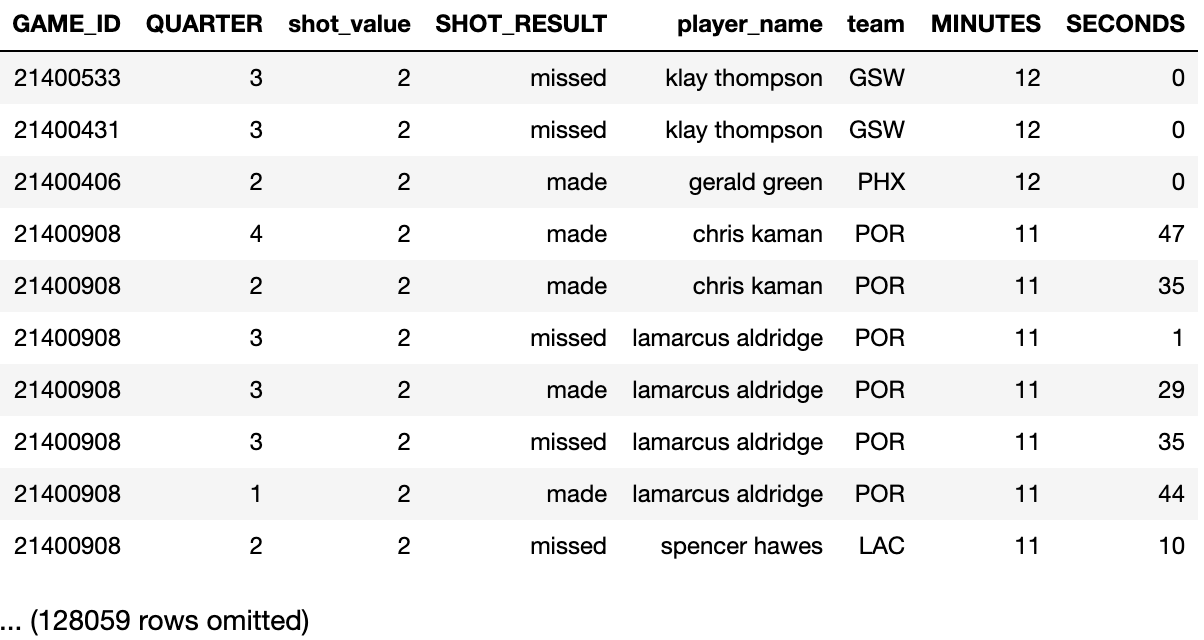
\includegraphics[scale=.6]{figures/shots_table.png}
\end{center}

\begin{enumerate}
\vskip 0.1in
\subq{2}
Write code to produce a table called \lsi+points+ that only contains shots that were "made" (points are only earned if a shot is made in the basket). The resulting table should have three columns: \lsi+GAME_ID+, \lsi+shot_value+, and \lsi+team+.
\vskip .2in
\solutionimage
{
\lstinline+points = shots.+\bklong
}
{
{\lsi+points = shots.where("SHOT_RESULT", are.equal_to("made")).select("GAME_ID", "shot_value", "team")+}
}
\vskip .1in
\subq{2} Assuming the \lsi+points+ table was implemented correctly, write code to produce a table \lsi+scores+ that contains the total number of points scored \textit{per team per game}. 

\vskip .2in
\solutionimage
{
\lstinline+scores = points.+\bkshort+(make_array(+\bkshort+, +\bkshort+), +\bkshort+)+
}
{
{\lsi+scores = points.group(make_array("GAME_ID", "team"), sum)+}
}
\vskip .1in
\subq{2} Assuming the \lsi+scores+ table was implemented correctly, write code to produce a table \lsi+sorted_scores+ where within each game (two rows with the same \lsi+GAME_ID+ but different teams), the row representing the team that scored the most points comes before the row representing the team that scored the least points. 
\vskip .2in
\solutionimage
{
\lstinline+sorted_scores = scores.+\bkshort+(+\bk+, +\bk+).sort("GAME_ID")+
}
{
{\lsi+sorted_scores = scores.sort("shot_value sum", descending = True).sort("GAME_ID")+}
}
\vskip .1in

\subq{4} Assuming the \lsi+sorted_scores+ table was implemented correctly, write code to produce a table called \lsi+win_count+, which should contain two columns:
\begin{itemize}
    \item \lsi+team+: The team name
    \item \lsi+count+: the number of games the team won
\end{itemize}

The team that won the most games should be the first row of the table.\newline
\vskip 0.1in
\solutionimage 
{
\lsi+winners_of_games = sorted_scores.+\bkshort+(np.arange(0,sorted_scores.num_rows,2))+\newline

\lsi+unsorted_winners = winners_of_games.+\bk+(+\bk+)+\newline

\lstinline+win_count = unsorted_winners.+\bk+(+\bk+, +\bk+)+
}
{
{\lsi+winners_of_games = sorted_scores.take(np.arange(0,sorted_scores.num_rows,2))+}\newline
{\lsi+unsorted_winners = winners_of_games.group("team")+}\newline
{\lstinline+win_count = unsorted_winners.sort("count", descending=True)+}

}


\end{enumerate}
      \clearpage
      \q{12}{Boba Distributions}

Anna is curious about her boba spending habits. The following is a histogram of her weekly spending on boba, over the span of \textbf{50} weeks (she doesn’t drink boba on her yearly two week vacation): 
%FIXME Do we like placement of hist? 
\begin{center}
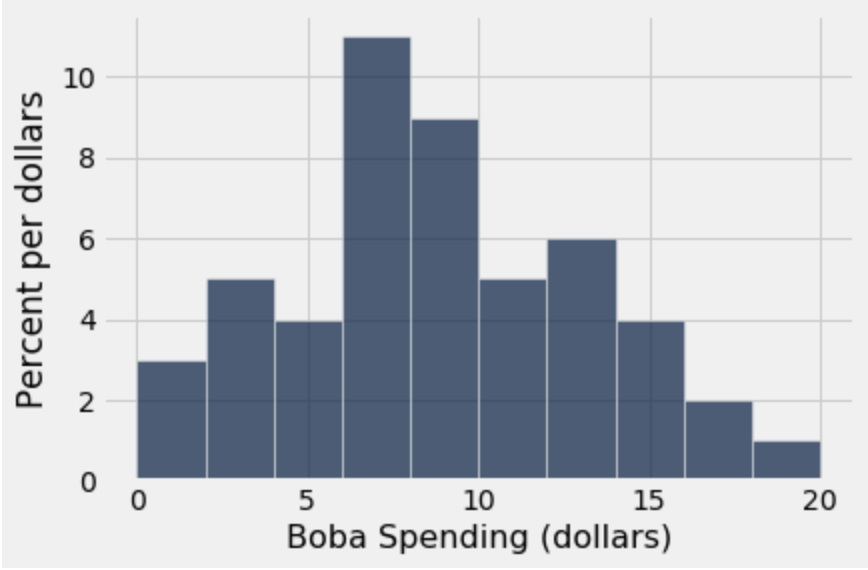
\includegraphics[scale=.6]{q3_boba}
\end{center}
The spending is divided into bins of width 2: [0,2), [2,4) ... [18,20).  

Assume that all of the data is shown on the histogram (Anna never spent \$20 or more in a given week).  

For the following questions, write a \textbf{mathematical expression} for the answer, or write \textit{“Not possible”} if it is not possible to calculate the desired quantity with the information in the given histogram.

\begin{enumerate}
\vskip .2in
% Do we want to bold percent? 
\subq{3} In what percent of weeks did Anna spend \$16 or more on boba?

\solution{2*2 + 1*2 = 6\%}

\vskip .6in
% Do we want to bold percent? 
\subq{3} In what percent of weeks did Anna spend between \$12 and \$15 on boba? 

\solution{Not possible to determine}

\vskip .6in
\subq{3} During how many weeks did Anna spend between \$10 and \$13 dollars?

\vskip 0.1in
\begin{tabular}{l@{\hskip 1in}l@{\hskip 1in}l@{\hskip 1in}l}
\bubble\quad 11 weeks \\
\solutionbubble \quad Between 5 and 11 weeks \\
\bubble \quad 22 weeks \\
\bubble \quad Between 10 and 22 weeks \\
\bubble \quad Not possible to calculate using the histogram
\end{tabular}

\vskip .2in
\subq{3} After looking over her notes, Anna finds that she entered the wrong data for two of the weeks when constructing the histogram. She is not sure whether her spending in those weeks should go in the [12, 14) or [14, 16) bin, so she decides to combine all of the data in those two bins into one bin of width 4, from [12,16). What is the height of this new bin? 

\solution{(0.6*2 + 0.4*2)/4 = 5 \%/\$}


\end{enumerate}

      \clearpage
      \q{22}{Don't Count Your Chickens}\\[10pt]
You're an avid chicken farmer. You built two coops for two groups of chickens (your Bantams, which lay small eggs, and your Jersey Giants, which lay big eggs) since you think they would prefer different sized nesting boxes. Unfortunately, when you visit your coops during the day, you are dismayed to see that it seems like chickens choose coops at random to spend time in, and your hard work was for nothing.\\[5pt]
However, your data scientist friend helps you collect eggs one morning and notices that the eggs in one coop seem to tend to be larger than the eggs in the other! Perhaps the chickens do show preference in where they sleep at night and lay their eggs. Overjoyed, you decide to investigate: one morning, after all the chickens have exited their coops, you measure the weight of each egg, and record in which coop it was found. 
You create the following table called \lsi+eggs+ to store the data, and then plot this histogram to help you visualize the difference:
\vskip 0.2 in
% \begin{center}
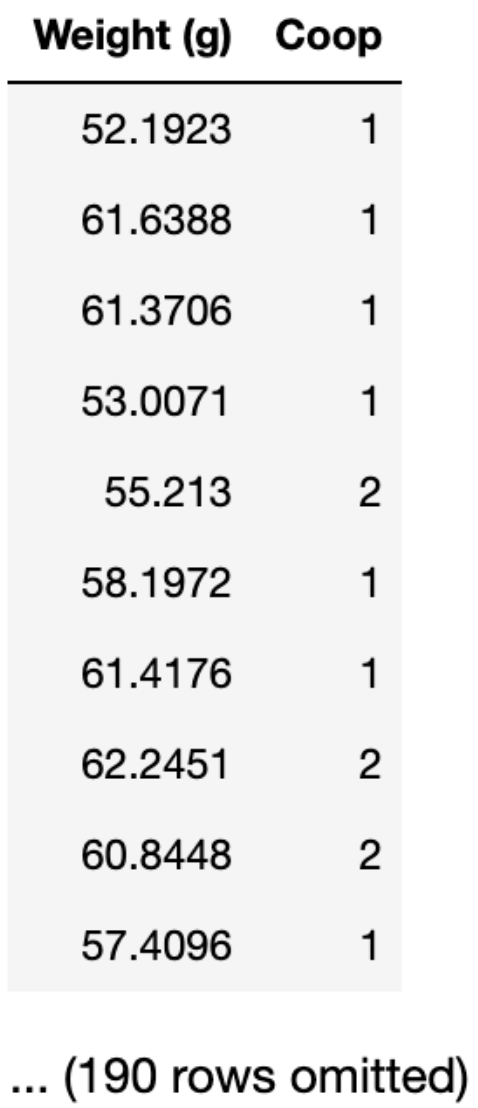
\includegraphics[scale=.35]{figures/chicken_table.png}
% \end{center}
% \begin{center}
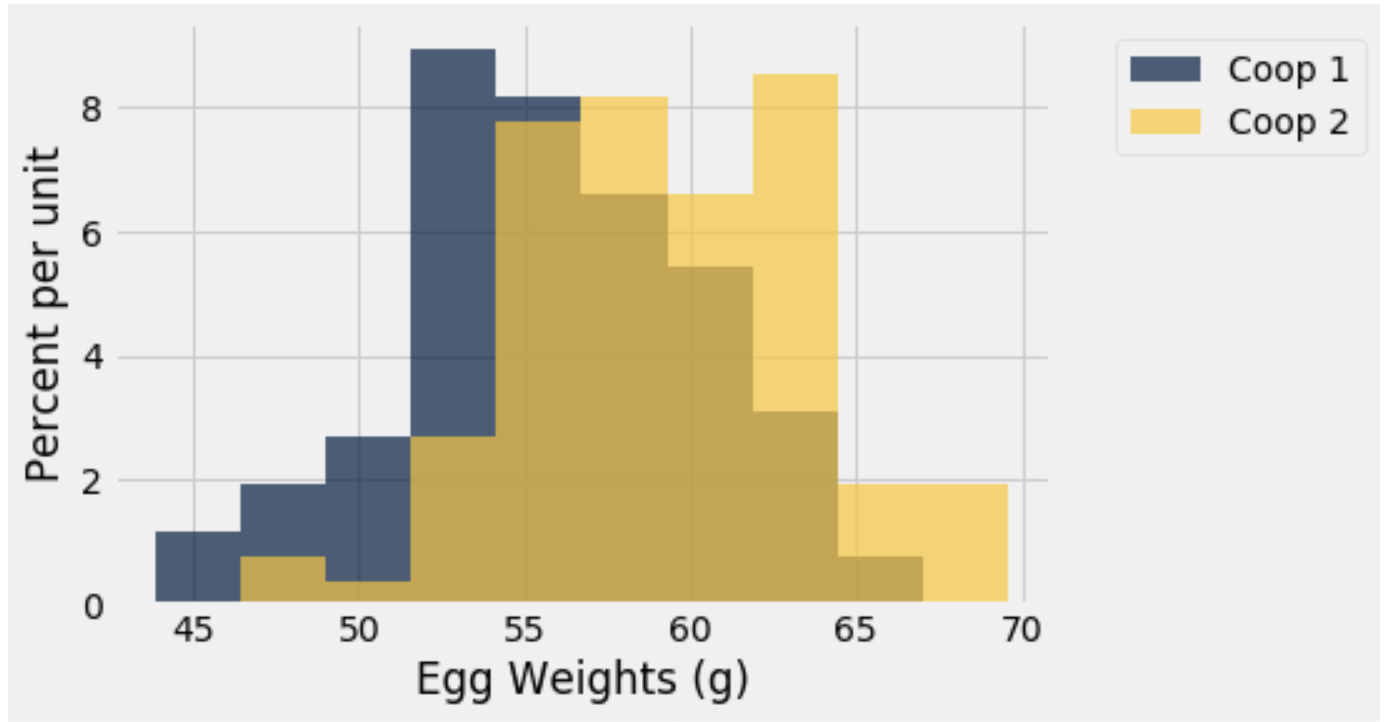
\includegraphics[scale=.55]{figures/chicken_hist.png}
% \end{center}
\vskip 0.2in
You want to conduct a hypothesis test to see if the distributions of egg weights come from one underlying distribution and thus support the idea that your chickens have no coop preference, or if instead the distributions of egg weights in the two coops are truly different. 

\vskip .05in
\begin{enumerate}

\subq{2} If we took a single bootstrapped resample of the Coop 1 eggs, what would the histogram of egg weights in our resampled table look like? 
\vskip 0.05in
\begin{enumerate}
    \bubble \quad The histogram would look like the Coop 1 histogram above, but narrower.\\[2pt]
    \bubble \quad The histogram would look like the Coop 1 histogram above,  but more normal.\\[2pt]
    \bubble \quad The histogram would be like the Coop 1 histogram above, but wider.\\[2pt]
    \solutionbubble \quad The histogram would not change very much from the Coop 1 histogram above. 
\end{enumerate}

\vskip .1in
\subq{2} How would you perform a single simulation under the null hypothesis that the distribution of weights in the two coops is the same?
\vskip 0.05in
\begin{enumerate}
    \bubble \quad Create two normal distributions centered at the mean of Coop 1 and Coop 2 and see if they overlap.\\[2pt]
    \solutionbubble \quad Shuffle the coop labels of your collected eggs and compute your test statistic on the shuffled table.\\[2pt]
    \bubble \quad Bootstrap the egg weights and calculate a new average egg weight.
\end{enumerate}

\vskip 1in    
\subq{2} What test statistic would \textbf{best} help differentiate between the null and the alternative hypothesis?
\vskip 0.05in
\begin{enumerate}
    \bubble \quad The Total Variation Distance (TVD) between the distribution of Coop 1 egg weights and Coop 2 egg weights. \\[2pt]
    \solutionbubble \quad The absolute value of the difference between the mean egg weight in Coop 1 and the mean egg weight in Coop 2.\\[2pt]
    \bubble \quad The mean egg weight of Coop 2.\\[2pt]
    \bubble \quad The difference between the mean egg weight in Coop  2 and Coop 1.
\end{enumerate}

\vskip .1in
\subq{4} Write a function \lsi+compute_one_test_stat+ that will take in the table with the same columns as \lsi+eggs+ above and returns one simulated value of your test statistic.
\vskip 0.05in
\solutionimage
{
{\lsi+def compute_one_test_stat(tbl):+}\\[10pt]
    \hspace*{0.5in}{\lsi+new_labels = +\bklong}\\[10pt]
    \hspace*{0.5in}{\lsi+new_table = +\bklong}\\[10pt]
    \hspace*{0.5in}{\lsi+means_col = +\bkshort+.+\bkshort+(+\bkshort+, +\bkshort+).+\bklong}\\[10pt]
    \hspace*{0.5in}{\lsi+test_stat = +\bklong}\\[10pt]
    \hspace*{0.5in}{\lsi+return test_stat+}
}
{
{\lsi+def compute_one_test_stat(tbl):+}\\[10pt]
    \hspace*{0.5in}{\lsi+new_labels = tbl.sample(with_replacement=False).column("Coop")+}\\[10pt]
    \hspace*{0.5in}{\lsi+new_table = tbl.with_columns("Shuffled labels", new_labels)+}\\[10pt]
    \hspace*{0.5in}{\lsi+means_col = new_table.group("Shuffled labels", np.mean).column('Weight (g) mean')+}\\[10pt]
    \hspace*{0.5in}{\lsi+test_stat = abs(means_col.item(0) - means_col.item(1))+}\\[10pt]
    \hspace*{0.5in}{\lsi+return test_stat+}
}
\vskip 0.1in
\subq{2} You use the \lsi+compute_one_test_stat+ function to compute the observed test statistic, which is stored in the variable \lsi+obsv_test_stat+, as well as 10,000 simulated test statistics,  which are stored in an array called \lsi+stats+.  Which of the following lines of code correctly computes the empirical p-value of this test? 
\vskip 0.05in
\begin{enumerate}
    \bubble \quad \lsi+np.count_nonzero(stats <= obsv_test_stat)/10000+\\[2pt]
    \solutionbubble \quad \lsi+np.count_nonzero(stats >= obsv_test_stat)/10000+\\[2pt]
    \bubble \quad \lsi+np.count_nonzero(stats == obsv_test_stat)/10000+\\[2pt]
    \bubble \quad \lsi+np.count_nonzero(stats >= 0.05)/100000+\\[2pt]
\end{enumerate}

\subq{4} \textbf{Select one of the options from parts i-ii to fill in the corresponding blanks in the sentence below.}

A larger observed difference in mean egg sizes would result in a \underline{\hspace{0.25in}}(i)\underline{\hspace{0.25in}} p-value. We would see a larger observed difference in mean egg sizes if Jersey Giant chickens exhibited a  \underline{\hspace{0.25in}}(ii)\underline{\hspace{0.25in}} preference for one coop, e.g. Coop 2.
\vskip 0.1in
\begin{enumerate}
    \item 
        {\solutionbubble} smaller\hspace{0.25in} {\bubble} larger
    \item
        {\bubble} weaker \hspace{0.25in}{\solutionbubble} stronger
\end{enumerate}

\vskip 0.1in
\subq{6} You calculate a p-value of 0.04 for this test. Select \textbf{all} true statements that we can justifiably conclude from this p-value. If you do not have enough information to evaluate whether the statement is true or false, DO NOT select it.
\vskip 0.05 in
\checkbox  There is a 4\% chance that the chickens have no preference for which coop they lay eggs in. \\
\checkbox  There is a 96\% chance that the chickens have no preference for which coop they lay eggs in.\\
\checkbox  If chickens actually have no coop preference, there is a 4\% chance we incorrectly reject the null hypothesis. \\
\solutionbox  We would reject the hypothesis that the chickens have no coop preference if we used a 5\% p-value cutoff.\\
\solutionbox   We would fail to reject the hypothesis that the chickens have no coop preference if we used a 1\% p-value cutoff.\\
\solutionbox   4\% of the simulated test statistics were greater than or equal to the observed test statistic.\\
\checkbox We cannot conclude any of the above options.

\end{enumerate}

      \clearpage
      \q{14}{I'll Take Civic Participation for 100 Points Please}
\vskip 0.1 in
A Berkeley political science professor is concerned about their students' knowledge of current U.S political events. To assess their civic participation, the professor sent a survey to 150 randomly-selected students quizzing them on their knowledge of recent news out of a total score of 100. In the 150-student sample, the mean score was 71.7 and standard deviation was 6.2. Here is a plot of the distribution of the 150 scores:

\begin{center}
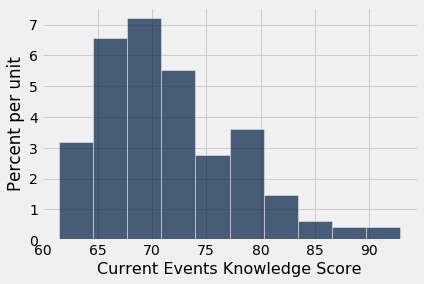
\includegraphics[scale=.7]{figures/civic_hist.png}
\end{center}

\textbf{For parts a - c, choose the option that best completes the blank.}
\vskip .1in
\begin{enumerate}
\subq{2} This distribution is \lsi++\bk++.
\vskip 0.1in
	\bubble \quad Left skewed\newline
	\solutionbubble \quad Right skewed\newline
	\bubble \quad Normally distributed
\vskip 0.2in
\subq{2} The mean of the above histogram is \lsi++\bk++ the median.
\vskip 0.1in
	\solutionbubble \quad higher than\newline
	\bubble \quad lower than\newline
	\bubble \quad equal to

\vskip 0.2in
\subq{2} The professor can expect at least \lsi++\bkshort++ of the scores to be between 59.3 and 84.1. 
\vskip 0.1in
	\bubble \quad 95\%\newline
	\bubble \quad 89\%\newline
	\solutionbubble \quad 75\%\newline
	\bubble \quad We don't have enough information to tell.
\clearpage
Although the professor only ended up with 150 entries for the survey, the professor decided to assume that this distribution of survey scores is representative of the entire  UC Berkeley student population. To get a better estimate of the entire student population’s knowledge, the professor conducts the following analysis:
\vskip 0.1in
\begin{itemize}
\item The professor resamples 150 scores with replacement from the original survey distribution.
\item The professor calculate the average of those 150 scores and store it in an array called \lsi+scores+. 
\item The professor repeat the above process 10,000 times.
\end{itemize}
\vskip 0.1in
Thus, \lsi+scores+ is an array of 10,000 average survey scores.
\vskip 0.2in
\subq{2} If the professor graphed the \lsi+scores+ distribution as a histogram, what would the shape of the histogram look like?
\vskip 0.1in
\begin{tabular}{l@{\hskip 1in}l@{\hskip 1in}l@{\hskip 1in}l}
\bubble \quad Left skewed
&\bubble \quad Right skewed\\[6pt]
\solutionbubble \quad Normally distributed
&\bubble \quad We don't have enough information to tell.
\end{tabular}

\vskip 0.2in
\subq{2} If the professor graphed the \lsi+scores+ distribution as a histogram, which of the following would be the best approximation of the mean/center of the distribution?
\vskip 0.1in
\begin{tabular}{l@{\hskip 1in}l@{\hskip 1in}l@{\hskip 1in}l}
\bubble \quad 7.17
 &\solutionbubble \quad 71.7  \\[6pt]
\bubble \quad 50
&\bubble \quad We don't have enough information to tell.
\end{tabular}

\vskip 0.22in
\subq{2} If the professor graphed the \lsi+scores+ distribution as a histogram, which of the following is the best approximation for the standard deviation of the distribution?
\vskip 0.1in
\begin{tabular}{l@{\hskip 1in}l@{\hskip 1in}l@{\hskip 1in}l}
\bubble \quad 6.2
&\solutionbubble \quad ${\displaystyle \frac{6.2}{\sqrt{150}} }$\\[6pt]
\bubble \quad ${\displaystyle \frac{\sqrt{150}}{6.2}}$
&\bubble \quad We don't have enough information to tell.
\end{tabular}

\vskip 0.2in
\subq{2} Still looking at the \lsi+scores+ distribution (i.e. the distribution of average survey scores), if we take only the average scores that are 1 SD of sample means away from the true average, roughly how much of the data (average survey scores) would we be looking at? 
\vskip 0.1in
\begin{tabular}{l@{\hskip 1in}l@{\hskip 1in}l@{\hskip 1in}l}
\bubble \quad 10\%
&\solutionbubble \quad 68\%\\[10pt]
\bubble \quad 75\%
&\bubble \quad 95\%
\end{tabular}
\end{enumerate}
      \clearpage
      \q{16}{Knowledge versus Participation}
\vskip .2 in
Berkeley is an interdisciplinary place! A rhetoric professor has been collecting data on students' use of social media to discuss current events, and decides to combine her data with the political scientist's data in the previous question. The data are not anonymous, so the professors are able to link student's current events knowledge scores to a "participation factor" (a continuous value from 0 to 10) that assesses how often students engage with political causes online. 
The following is a scatter plot of the current events knowledge scores  (from question 5) versus the participation factor. 
\begin{center}
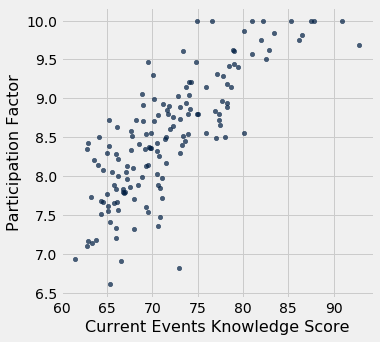
\includegraphics[scale=.8]{figures/regression_scatter.png}
\end{center}
Here is some summary information about the data:
\begin{itemize}
    \item The average current events knowledge score is 71.7, and the standard deviation of the current events knowledge score is 6.2. 
    \item The average participation factor was 8.5, and the standard deviation of the participation factor is 0.78.
    \item The correlation coefficient between current events knowledge and the participation factor across the 150 students is 0.8.
\end{itemize}

\begin{enumerate}
\subq{2} What is the slope of the least squares regression line predicting participation factor from current events knowledge score? Do not simplify your answer (show your work!).\\
\solution{$0.8 \times \frac{0.78}{6.2}$}
\vskip 0.5in
\subq{2} What is the intercept of the least squares regression line predicting participation factor from current events knowledge score? Do not simplify your answer (show your work!).\\
\solution{$8.5 - (0.8 \times \frac{0.78}{6.2})\times 71.7$}
\clearpage
\subq{6} The rhetoric professor plotted three lines on the scatter plot. They then plotted the errors between these lines and the data. \textbf{Match the three lines (A, B, C) to their corresponding error plots.} One error plot does not have a matching line.
\vskip 0.1in

\begin{center}
    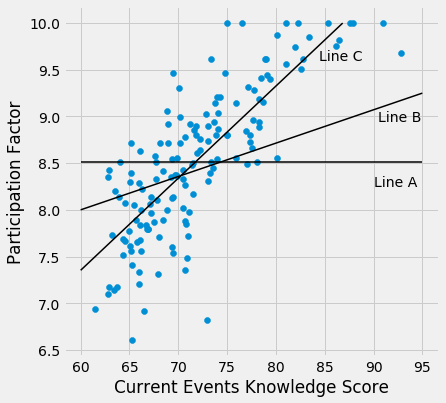
\includegraphics[scale=.42]{figures/regression_lines.png}
    \\[8pt]
    \textbf{Pick one of the bubbles for each of the following error plots.}
\end{center}
\vskip 0.1in
\begin{tabular}{l@{\hskip 0.8in}l@{\hskip 0.1in}l@{\hskip 0.1in}l}
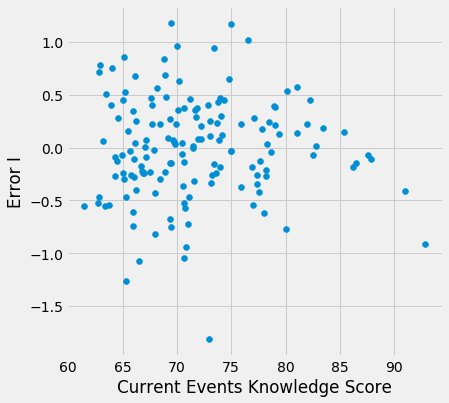
\includegraphics[scale=.41]{figures/residuals.png}
&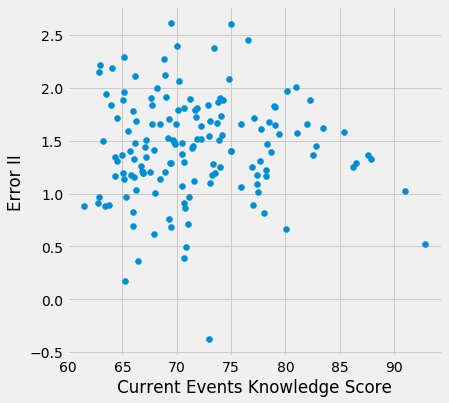
\includegraphics[scale=.41]{figures/wrong_error_b.png}
\\[2pt]
%solutions for first two plots
\begin{tabular}{l@{\hskip 0.5in}l@{\hskip 0.1in}l@{\hskip 0.1in}l}
&\bubble Line A{\hskip 0.1in}&\bubble Line B{\hskip 0.1in}\\ &\solutionbubble Line C{\hskip 0.1in}&\bubble No match
\end{tabular}
&\begin{tabular}{l@{\hskip 0.5in}l@{\hskip 0.1in}l@{\hskip 0.1in}l}
&\bubble Line A{\hskip 0.1in}&\bubble Line B{\hskip 0.1in}\\ &\bubble Line C{\hskip 0.1in}&\solutionbubble No match
\end{tabular}\\[18pt]

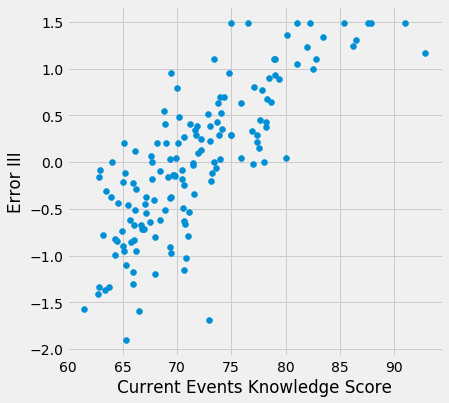
\includegraphics[scale=.41]{figures/error_from_average.png}
&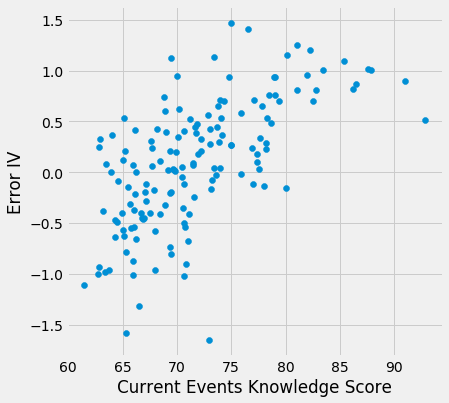
\includegraphics[scale=.41]{figures/error_from_bad_line.png}\\[2pt]

%solutions for second two plots
\begin{tabular}{l@{\hskip 0.5in}l@{\hskip 0.1in}l@{\hskip 0.1in}l}
&\solutionbubble Line A{\hskip 0.1in}&\bubble Line B{\hskip 0.1in}\\ &\bubble Line C{\hskip 0.1in}&\bubble No match
\end{tabular}
&\begin{tabular}{l@{\hskip 0.5in}l@{\hskip 0.1in}l@{\hskip 0.1in}l}
&\bubble Line A{\hskip 0.1in}&\solutionbubble Line B{\hskip 0.1in}\\ &\bubble Line C{\hskip 0.1in}&\bubble No match
\end{tabular}
\end{tabular}


\vskip 0.2in
\subq{2} One of the three lines in the plot in part \textbf{c} is the least squares regression line, and one line is the line \textit{predicted y = average(y)}. Which one is which? 
\vskip 0.1in
\begin{center}
\textbf{Least Squares Regression Line}
\vskip 0.1in
\begin{tabular}{l@{\hskip 0.3in}l@{\hskip 0.3in}l@{\hskip 0.3in}l}
\bubble Line A
&\bubble Line B
&\solutionbubble Line C
\end{tabular}
\vskip 0.2in
\textbf{\textit{predicted y = average(y)}}
\vskip 0.1in
\begin{tabular}{l@{\hskip 0.3in}l@{\hskip 0.3in}l@{\hskip 0.3in}l}
\solutionbubble Line A
&\bubble Line B
&\bubble Line C
\end{tabular}
\end{center}
\vskip 0.25in
\subq{1} Rank the mean squared error of the three lines from smallest to largest:
\vskip 0.1in
\begin{tabular}{l@{\hskip 0.5in}l@{\hskip 0.5in}l@{\hskip 0.5in}l}
\bubble A, B, C
&\bubble B, C, A
&\bubble A, C, B\\[6pt]
\bubble B, A, C
&\bubble C, A, B
&\solutionbubble C, B, A

\end{tabular}
\vskip 0.25in
\subq{3} Select \textbf{all} true statements we can justifiably conclude. If you do not have enough information to evaluate whether the statement is true or false, DO NOT select it.
\vskip 0.1in
\solutionbox The root mean squared error (RMSE) of line A is equal to the standard deviation of the participation score.
\vskip 0.1in
\checkbox The root mean squared error of line B is equal to the standard deviation of the fitted values from line B.
\vskip 0.1in
\solutionbox The root mean squared error of line C is equal to the standard deviation of the residuals. 
\vskip 0.1in
\solutionbox It is impossible to create a linear model that will give you a smaller root mean squared error than the root mean squared error from line C.

\end{enumerate}
      \vskip 0.4in
      \q{12}{Some More Regression}
\begin{enumerate}
    \vskip 0.2in
    \subq{3} The following depicts a scatter plot between two numerical variables (labeled \textit{x} and \textit{y}). A line (labeled "Line A") has been drawn through the scatter plot, but note that Line A is not the least squares regression line between x and y. \textbf{On the plot itself (do not make a separate plot), draw a line with a \textit{larger} root mean square error than the existing line.}
    \vskip 0.2in
    \begin{center}
        \solutionimage
        {
        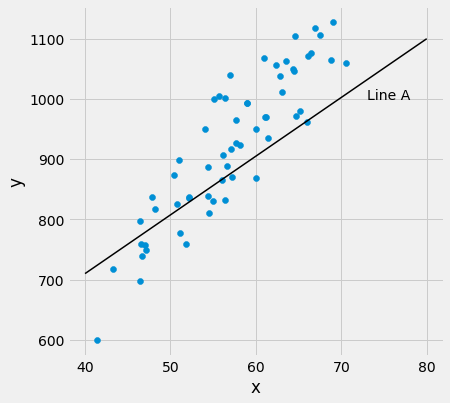
\includegraphics[scale=.45]{figures/labelledporpourri.png}
        }
        {
        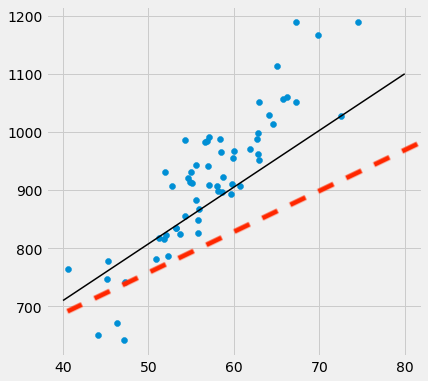
\includegraphics[scale=.45]{figures/potpourri_plot_sol.png}
        \solution{The line at left is one example of a valid answer.}
        }
    \end{center}
    
    
    

    \clearpage
    \subq{6} We have provided three empty plots, with axes in standard units. Draw a dataset of ten to twenty points with the specified value for \textit{r}. Make sure your points are clearly visible and large enough to see when scanned.\\[8pt]
    \textbf{Plot A:} Draw data points in a scatter plot such that the correlation of the points could be close to \textbf{0.}\\
    \textbf{Plot B:} Draw data points in a scatter plot such that the correlation of the points could be close to \textbf{0.99.}\\
    \textbf{Plot C:} Draw data points in a scatter plot such that the correlation of the points could be close to \textbf{-0.5.}\\
    \vskip 0.4in
    \solutionimage
    {
    \begin{tabular}{l@{\hskip 1in}l@{\hskip 0.1in}l@{\hskip 0.1in}l}
    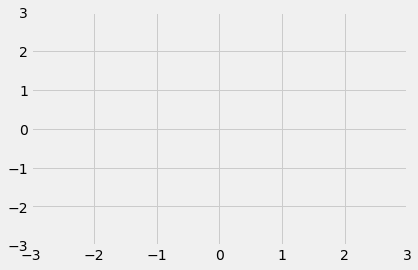
\includegraphics[scale=.45]{figures/blankaxes.png}
    &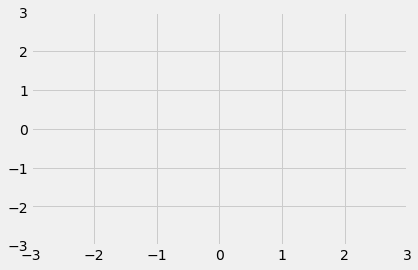
\includegraphics[scale=.45]{figures/blankaxes.png}\\
    {\hskip 1in}\textbf{Plot A}
    &{\hskip 1in}\textbf{Plot B}
    \end{tabular}
    \begin{center}
        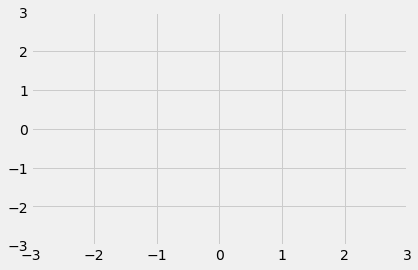
\includegraphics[scale=.45]{figures/blankaxes.png}\\
        \textbf{Plot C}
    \end{center}
    \solution{The points above are examples of valid solutions.}
    }
    {
    \begin{tabular}{l@{\hskip 1in}l@{\hskip 0.1in}l@{\hskip 0.1in}l}
    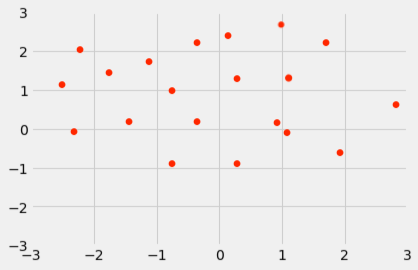
\includegraphics[scale=.45]{figures/corr0soln.png}
    &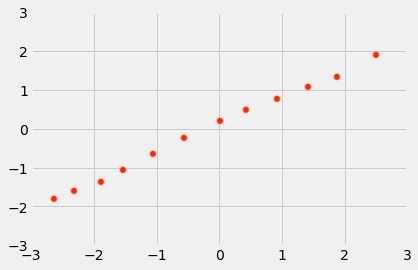
\includegraphics[scale=.45]{figures/corr099soln.png}\\
    {\hskip 1in}\textbf{Plot A}
    &{\hskip 1in}\textbf{Plot B}
    \end{tabular}
    \begin{center}
        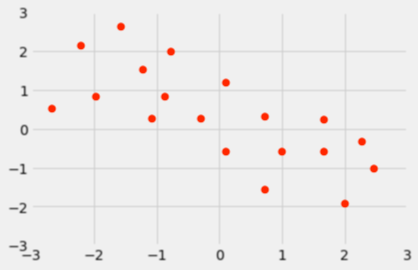
\includegraphics[scale=.45]{figures/corrneg05soln.png}\\
        \textbf{Plot C}
    \end{center}
    \solution{The points above are examples of valid solutions.}
    }
    \vskip 0.4in

    \subq{3} A researcher is interested in the relationship between the number of bumblebees and the number of ground squirrels observed in an alpine meadow over the course of one day. They calculate the regression line between the number of bees and the number of squirrels, and finds that the slope of the regression is 0.0314. Curious about the small value of the slope, the researcher wants to test the following hypotheses: 
    \begin{itemize}
        \item Null: The slope of the true line describing the relationship between number of bees and  number of squirrels in alpine meadows is zero. 
        \item Alternative: The slope of the true line describing the relationship between between number of bees and  number of squirrels in alpine meadows is not zero.
    \end{itemize}
The researcher finds that an  approximate 90\% confidence interval for the true slope is [0.013, 0.045]. Select \textbf{all} the p-value cutoffs for which the researcher will reject the null hypothesis:
\vskip 0.1in
\solutionbox 20\%\\
\solutionbox 10\%\\
\checkbox 5\%\\
\checkbox 1\%\\

\end{enumerate}
      \clearpage
      \q{24}{Rock Solid Confidence}\\[10pt]
A petrologist (someone who studies rocks) has collected a random sample of 500 sandstone rocks from a desert region. They are interested in knowing the mean density of sandstone rocks in that region. They find that the mean density of the sample is 2.4 grams/cm$^3$. Instead of giving just one estimate, they wish to provide a range of values.

\begin{enumerate}
    \subq{6} \textbf{Select one of the options from each parts i-vi to fill in the corresponding blanks in the sentence below.}
    \vskip 0.05in
    The actual mean density of the sandstone rocks in the region is the population \underline{\hspace{0.25in}}(i)\underline{\hspace{0.25in}} . Rather than going back to the original population and taking a new sample, the scientist will use the sample they already have. This technique is known as bootstrapping.  To use the bootstrap method, the scientist will take many samples \underline{\hspace{0.25in}}(ii)\underline{\hspace{0.25in}} from the \underline{\hspace{0.25in}}(iii)\underline{\hspace{0.25in}} to create one bootstrapped sample. We find the \underline{\hspace{0.25in}}(iv)\underline{\hspace{0.25in}} of each bootstrap sample. After we've completed this process, we can compute a \underline{\hspace{0.25in}}(v)\underline{\hspace{0.25in}}. We are more confident that our procedure will generate an interval that captures the actual mean density when we use a \underline{\hspace{0.25in}}(vi)\underline{\hspace{0.25in}} interval.
    
        \vskip 0.1in
        
    \begin{enumerate}
        \item
            {\solutionbubble} parameter
            \hspace{0.25in}{\bubble} statistic
        \item
            {\bubble} without replacement
            \hspace{0.25in}{\solutionbubble} with replacement
        \item
            {\bubble} population
            \hspace{0.25in}{\solutionbubble} original sample
        \item
            {\bubble} middle 95\%
            \hspace{0.25in}{\solutionbubble} mean
        \item
            {\solutionbubble} confidence interval
            \hspace{0.25in}{\bubble} p-value
        \item
            {\solutionbubble} wider
            \hspace{0.25in}{\bubble} narrower
    \end{enumerate}
    \vskip 0.1in
    
    \subq{4} Select all of the following conditions under which bootstrapping would not be an effective estimation technique.
    \vskip .1in
    \begin{enumerate}
        \checkbox The original sample is very big.\\[2pt]
        \solutionbox You are trying to estimate the minimum value of a population.\\[2pt]
        \solutionbox The original sample is very small.\\[2pt]
    	\checkbox The original sample is a random sample from the population.\\[2pt]
        \checkbox You are trying to estimate the median value of a population.\\[2pt]
	    \checkbox The distribution of your population is not roughly bell shaped. \\[2pt]

    \end{enumerate}

    
    \subq{6} The table called \lsi+rocks+ has one column, \lsi+density+, containing the density of the 500 sampled rocks in the region. Write code such that \lsi+left_end+ and \lsi+right_end+ evaluate to the endpoints of a ninety percent \textbf{ (90\%)}  confidence interval for the mean density of rocks in the region using 10,000 bootstrapped resamples.
    \vskip .1in
    \solutionimage
    {
    {\lsi+means = +\bkmed++}\\[10pt]
    {\lsi+for+\bkmed+:+}\\[10pt]
    \hspace*{0.5in}{\lsi+resample =+\bklong}\\[10pt]
    \hspace*{0.5in}{\lsi+resample_mean =+\bklong}\\[10pt]
    \hspace*{0.5in}{\lsi+means =+\bklong}\\[10pt]
    {\lsi+left_end = +\bk+( 5 , +\bk+)+}\\[10pt]
    {\lsi+right_end = +\bk+(+\bkshort+, +\bk+)+}
    }
    {
    {\lsi+means = make_array()+}\\[10pt]
    {\lsi+for i in np.arange(10000):+}\\[10pt]
    \hspace*{0.5in}{\lsi+resample = rocks.sample()+}\\[10pt]
    \hspace*{0.5in}{\lsi+resample_mean = np.mean(resample.column("density"))+}\\[10pts]
    \hspace*{0.5in}{\lsi+means = np.append(means, resample_mean)+}\\[10pt]
    {\lsi+left_end = percentile(5, means)+}\\[10pt]
    {\lsi+right_end = percentile(95, means)+}\\[10pt]
    }
    

    \clearpage
    \subq{4} Select \textbf{all} answers that we can justifiably conclude. If you do not have enough information to evaluate whether the statement is true or false, DO NOT select it.
    \vskip .1in
    \begin{enumerate}
        \checkbox If the petrologist convinces 100 of their colleagues to independently take new random samples of 500 rocks, and each colleague generates one approximate 80\% confidence interval for the true mean rock density in the region,  about 95 of the 100 intervals will contain the true mean rock density of the region. \\[2pt]
        \solutionbox If the petrologist convinces 100 of their colleagues to independently take new random samples of 500 rocks, and each colleague generates one approximate 90\% confidence interval for the true mean rock density in the region,  about 90 of the 100 intervals will contain the true mean rock density of the region.\\[2pt] 
        \solutionbox If the petrologist's colleague runs the code from part (c), but changes the endpoints of the interval (in the last two lines) to the 0.5th and 99.5th percentile, the resulting interval will be wider than the petrologist's original interval. \\[2pt]
        \checkbox  If the interval calculated in part c) is [1.9g/cm$^3$, 2.8g/cm$^3$], there is a 90\% chance that the true mean rock density of the region is in that interval.
    \end{enumerate}
    \vskip 0.1in
    \subq{4} If the width of a 90\% confidence interval you calculated was 1 gram/cm$^3$, \textbf{what is an estimate of the standard deviation of the rock densities in the population} of rocks from which we drew our sample of size 500? 
    \vskip 0.1in
    The table below shows percentages of values in a certain range under the normal curve, in addition to those already in the exam reference guide.
    
    \begin{center}
    \begin{tabular}{c|c}
    {\bf Percent in Range} & {\bf Normal Distribution} \\ \hline
    average $\pm$ 1.3 SDs & about 80\% \\ \hline
    average $\pm$ 1.65 SDs & about 90\% \\ 
    \end{tabular}
    \end{center}
    \\[10pt]
    Show your calculations below. You should NOT simplify arithmetic expressions. Please draw a box around your final answer.
    
    \solution{$1 = 2 \times 1.65 \times \text{SD of sample means}$}\\[5pt]
    \solution{$\text{SD of sample means} = \frac{1}{3.3}$}\\[5pt]
    \solution{$\frac{1}{3.3} = \frac{\text{population SD}}{\sqrt{500}}$}\\[5pt]
    \solution{$\text{population SD} = \frac{\sqrt{500}}{3.3}$}
\end{enumerate}
      \clearpage
      \q{18}{Find My Falafel}\\[10pt]
Francie and Natalia both love falafel (a delicious fried chickpea snack), but they often argue about the best falafel in Berkeley. Natalia likes the falafel from Bongo Burger (BB)  and Flying Falafel (FF) equally, but Francie says the BB falafel are too small and dry compared to the good stuff at FF. The Data 8 summer staff are fed up with Francie and Natalia arguing about falafel during staff meetings, so they decide to collect falafel from each location and train a classifier to determine where future falafel come from. \\
The staff purchase 100 falafels, 50 from each of BB and FF, and measure
\begin{itemize}
    \item \lsi+size+ : diameter of falafel, in millimeters.
    \item \lsi+moisture+ : the moisture content of each piece, reported as a percentage (by weight)
\end{itemize}
The following is a plot of the 100 falafel and their two characteristics. Circles are Bongo Burger falafel and crosses are Flying Falafel falafel. 
\begin{center}
    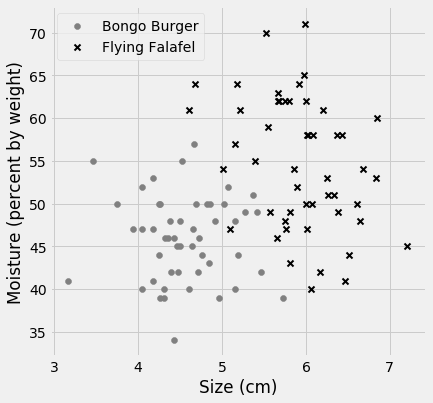
\includegraphics[scale=.6]{figures/falafel.png}
\end{center}

\begin{enumerate}
\subq{3} The two classes of falafel cannot be perfectly separated by a line on the plot above. Is it still appropriate to use k-nearest neighbors classification to classify the falafel?
    \vskip 0.1 in
    \solutionbubble \quad Yes, because k-nearest neighbors still works even if the data cannot be perfectly separated. \\[4pt]
    \bubble \quad Yes, because having individuals from different classes that overlap in their features allows you to use a higher value for k. \\[4pt]
    \bubble \quad Yes, because k-nearest neighbors transforms the data so that it can be separated by a decision boundary. \\[4pt]
    \bubble \quad No, because k-nearest neighbors does not work if the data cannot be perfectly separated. \\[4pt]
    \bubble \quad No, because the accuracy on the test set is guaranteed to be lower if the data cannot separated by a decision boundary. \\[4pt]

\clearpage
\textbf{Parts B and C refer to the information below.} \\
Natalia found another falafel on the ground. She wants to use the dataset we currently have to classify which restaurant the new falafel came from.  The following is an \textbf{unsorted } table of the seven pieces of falafel in our dataset closest (in terms of Euclidean distance between size and moisture content)  to the new piece of falafel:
\begin{center}
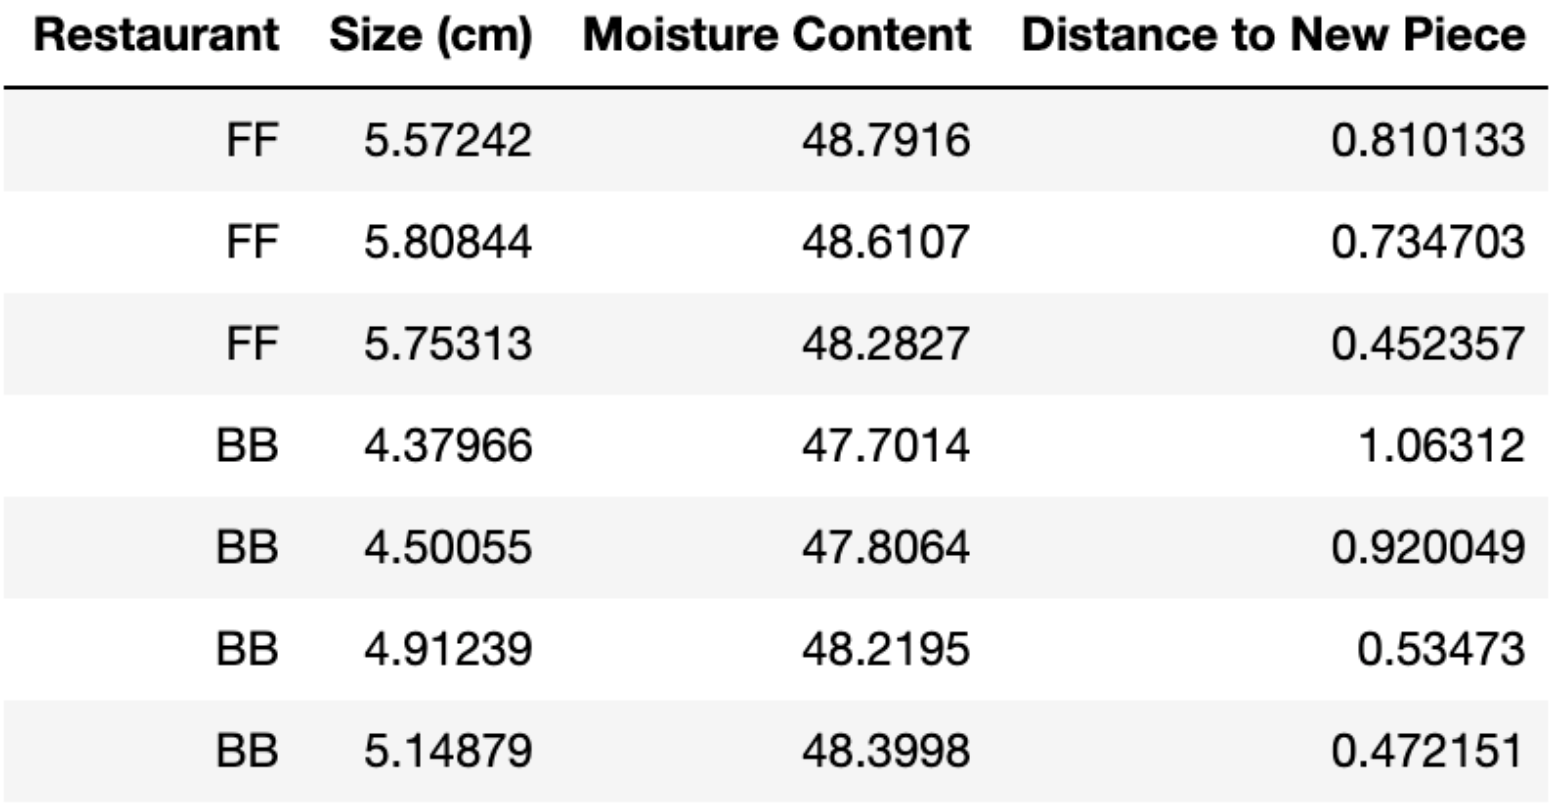
\includegraphics[scale=.34]{figures/falafel_nn.png}
\end{center}
\vskip0.1in
\subq{2} If we used a 3 nearest neighbor classifier, would we classify the new piece of falafel as coming from Bongo Burger or Flying Falafel?
\hspace{0.25in}\solutionbubble Bongo Burger\hspace{0.25in} \bubble Flying Falafel

\vskip .2in
\subq{2} If we used a 5 nearest neighbor classifier, would we classify the new piece of falafel as coming from Bongo Burger or Flying Falafel? 
\hspace{0.25in}\bubble Bongo Burger\hspace{0.25in} \solutionbubble Flying Falafel
\vskip0.1in
\subq{3} Shoumik is a visual learner and wrote out each step the classifier needs to perform on a different slip of paper and placed them on a desk. Before implementing the classifier Shoumik takes a break to teach his lab section. While he was gone, Shoumik's roommate rearranges the slips of paper while cleaning the desk, and now all the steps are out of order. Label the following steps as 1 ("do this first") to 6 ("do this last") in order to correctly implement a k nearest neighbors classifier. 
\vskip 0.1in
\solutionimage
{
{\underline{\qquad}} Take the top k rows of the sorted table\\[4pt]
{\underline{\qquad}} Calculate the classifier accuracy on all points in your test set\\[4pt]
{\underline{\qquad}} Classify the new point as the majority class in top k rows\\[4pt]
{\underline{\qquad}} Split the original data set into training and testing set\\[4pt]
{\underline{\qquad}} Sort the distances from smallest to largest\\[4pt]
{\underline{\qquad}} Calculate the distance between the new point and all points in the training set.
}
{
{\underline{\textbf{4}}} Take the top k rows of the sorted table\\[4pt]
{\underline{\textbf{6}}} Calculate the classifier accuracy on all points in your test set\\[4pt]
{\underline{\textbf{5}}} Classify the new point as the majority class in top k rows\\[4pt]
{\underline{\textbf{1}}} Split the original data set into training and testing set\\[4pt]
{\underline{\textbf{3}}} Sort the distances from smallest to largest\\[4pt]
{\underline{\textbf{2}}} Calculate the distance between the new point and all points in the training set.
}


\vskip 0.2in
\subq{2} Based on the scatter plot, which of the two features is more useful for differentiating falafel between the restaurants (e.g. if you could only use one feature to classify, which should you choose)? 
\vskip 0.03in
\hspace{0.25in}\bubble \quad moisture \hspace{0.25in} \solutionbubble \quad size
\vskip0.1in

\subq{3} The staff notice that falafel made in the morning are a different size than falafel made in the evening, as if restaurants are trying to conserve falafel batter at the end of the day. If you used a classifier trained on morning falafel to predict the label of an evening falafel, how might the accuracy of your classifier be affected? 
\begin{enumerate}
    \bubble \quad The test accuracy of your classifier would not change - you would do just as well using a classifier trained on morning falafel as a classifier trained on evening falafel.\\[2pt]
    \bubble \quad The test accuracy would increase because you are including more data.\\[2pt]
    \bubble \quad The test accuracy would increase because your accuracy would not depend on random variation in the morning falafel.\\[2pt]
    \solutionbubble \quad The test accuracy would decrease because the typical values of features for each restaurant might be different in the evening relative to the morning. 
\end{enumerate}

\vskip 0.2in
\subq{3} The staff decided to investigate evening falafel and created a new classifier using falafel collected in the evening. However, on the night of data collection Bongo Burger had a machine malfunction so the staff were only able to collect 10 BB falafel, and 90 FF falafel. A GSI tried many different values for \textit{k} (how many nearest neighbors to look at) when training their classifier, and noticed that above some value of \textit{k}, the classifier always classified any new falafel as coming from FF, regardless of its features. What is this value of \textit{k?} 
\vskip 0.1in
\begin{tabular}{l@{\hskip 0.5in}l@{\hskip 0.5in}l@{\hskip 0.5in}l}
\bubble \quad 11
&\bubble \quad 20 \\[10pt]
\solutionbubble \quad 21
&\bubble \quad 51
\end{tabular}



\end{enumerate}
      \vskip 0.8in
     \q{0}{Data art (optional)}
     Draw a visualization or graph describing your experience in Data 8.
     \vfill
      \q{0}
      {}Write your name in the space provided on one side of every page of the exam.
     You're done!
\end{enumerate}

\end{document}

